%%%%% Projekt z předmětu IMP %%%% 
%% Autor: (xcepel03)

\documentclass[]{fitiel} % dokumenty v~češtině, implicitní
\usepackage{hyperref}

% implicitní cesta k obrázkům
\graphicspath{{fig/}}

% hlavička 
% příkaz logo - vkládá logo fakulty dle zvoleného jazyka
\title{\logo
        \newline
        \\IMP -- protokol k projektu 15
        \\ARM-FITkit3 - Hra HAD}
\author{Kateřina Čepelková \\ xcepel03}
\date{\today}

\begin{document}
	\maketitle
    
    \newpage
	\tableofcontents

%%%%  Úvod do řešené problematiky
    \newpage
    \section{Úvod do řešené problematiky}
    Projekt byl naprogramován v~jazyce C v~prostředí Kinetis Design Studio.
    \\\\
    Úkolem bylo vytvořit obdobu hry "Had" na mikroprocesoru FITkit v3.0 s~přidaným modulem dvou maticových LED displejů (KWM-30881AGB). Ty jsou připojeny k mikroprocesoru FITkit v3.0 pomocí konektoru P1 na dané platformě a konektoru P3 na modulu s~displeji.
    \\\\
    Modul obsahuje LED diody uspořádané do řádků a sloupců. Tyto diody vydávají zelené světlo. Diody v~jednom řádku mají společný anodový vývod. Diody v~jednom řádku lze rozsvítit díky aktivaci řádkového vodiče (přivedením log. 1) a sloupcových vodičů (přivedením log. 0). Řádkový vodič je realizován pomocí demultiplexoru, neboli dekodéru 4-na-16. Výběr konkrétního sloupce je řešen pomocí řídících vstupů A0-A3.
    
%%%%  Způsob realizace
    \newpage
    \section{Způsob realizace}
    Jako první je v~kódu zavolána funkce \verb|void SystemConfig()|, která nakonfiguruje všechny potřebné periferie. Těmi jsou například hodiny, piny displejového modulu pro funkcionalitu GPIO a piny tlačítek \verb|(SWn)|.
    \\\\
    Následně je zavolána funkce \verb|void game()|, ve které je implementována hra. Nastavuje se zde počáteční pozice hada. Dále se zde nachází nekonečná smyčka. Ve zmíněné smyčce je volána funkce \verb|void| \verb|display_snake()|, která slouží ke zobrazování hada na maticovém displeji. Zobrazení probíhá pomocí 3 vnořených cyklů \verb|for|. Vnější cyklus stanovuje dobu zobrazení jednoho stavu hada. Druhý iteruje skrze všechny sloupce a aktivuje je pomocí funkce \verb|void column_select(unsigned int col_num)|. Třetí rozsvěcuje pouze konkrétní řádky, na kterých se vyskytuje had v~daném sloupci pomocí funkce \verb|void row_select(int row_pos)|. Díky těmto třem cyklům hra lidskému oku přijde jakoby viděl 5 svítících pixelů. Ve skutečnosti ale tyto pixely pouze velmi rychle problikávají. Ve funkci \verb|void|  \verb|display_snake()| se také sbírají informace o stisku tlačítka. To probíhá pomocí signálů zaslaných stiskem tlačítka uživatelem a informací o posledním známém směru, který zabraňuje uživateli couvat zpátky do těla hada.
    \\\\
    Po získání signálu o změně směru je aktualizována proměnná \verb|currentDirection|, která je realizována pomocí výčtového typu \verb|enum Direction {UP, DOWN, LEFT, RIGHT, NONE}|. Prvotní stav \verb|currentDirection| je \verb|NONE| a díky tomu je had na začátku hry nehybný. Po získání signálu je pomocí přepínače \verb|switch()| aktualizován nový směr na základě získaného vstupu. Had v~tomto směru pokračuje do té doby, než získá jiný signál, či je ukončena hra. Hra může být ukončena pokud se had bude snažit vstoupit mimo displej, nebo pokud se snaží vstoupit na políčko, které již okupuje. Obě tyto věci jsou kontrolovány ve funkci \verb|bool can_move()|, která vrací hodnotu \verb|true|, pokud je vše v~pořádku a had se může pohnout na novou pozici. V opačném případě vrací hodnotu \verb|false|.
    \\\\
    Had je realizován pomocí kruhového bufferu \verb|struct coords snake[5]| pro snadnější a efektivnější manipulaci. Struktura \verb|coords| obsahuje 2 datové typy \verb|int| pro uložení pozice na řádku (\verb|row|) a ve sloupci (\verb|col|).
    \\\\
    Funkce \verb|void game()| slouží také k resetování hry do prvotní pozice poté, co ji uživatel prohraje.  

%%%%  Výsledky a vlastnosti řešení
    \newpage
    \section{Výsledky a vlastnosti řešení}
    \subsection{Implementované vlastnosti:}
    \begin{itemize}
        \item Možnost konce hry -- pokud had "narazí" do zdi či do svého článku
        \item Omezení pohybu -- nelze couvat (otočit hlavu zpět do těla)
        \item Kontinuální pohyb ve vybraném směru do chvíle, než uživatel vybere jiný směr (pokračování kontinuálního pohybu v~tomto směru)
    \end{itemize}


    \subsection{Detailní popis vlastností:}
    Finální hra funguje tak, že po spuštění FITkitu s~nahranou aplikací se uživateli zobrazí nehybný had o délce 5 pixelů na pozicích {3, 10}, {3, 9}, {3, 8}, {3, 7}, {3, 6}, což je zhruba uprostřed displeje. 
    \\\\
    Hra začne až po stisku jednoho ze 3 tlačítek - levého, pravého či horního. Had totiž začíná v~pozici čelící nahoru, takže nemůže být jeho první pohyb dolů. Po stisku tlačítka se tedy had začne pohybovat ve vybraném směru korespondující jeho tlačítku. Had pokračuje ve vybraném směru dokud uživatel nestiskne jiné tlačítko (kromě opačného směru).
    \\\\
    Hra končí pokud uživatel narazí do zdi (= konec displeje) či do nějaké části jeho těla. Po skončení se hra obnoví do startovní pozice a uživatel může začít hrát znovu.

    \begin{figure}[h]
      \centering
      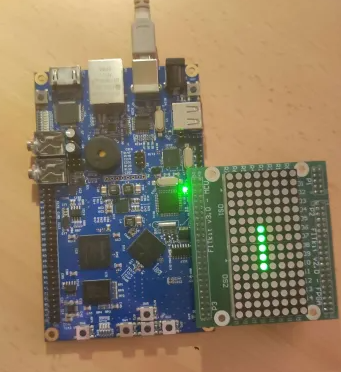
\includegraphics{fig/start.png}
      \caption{Začáteční stav hry}
    \end{figure}

%%%%  Vlastní zhodnocení
    \newpage
    \section{Vlastní zhodnocení}
    \subsection{E - Přístup}
    \textbf{1 bod}
    \\\\
    Projekt jsem začala dělat s~třítýdenním předstihem poté, co jsem skončila se všemi cvičeními z předmětu IMP, abych měla co nejširší předešlou praxi v~programování mikroprocesorů. 
    \\\\
    Snažila jsem se o co nejkvalitnější výstup s~pokrytím všech okrajových případů a jejích nápaditým řešením - např. restart hry.
    \subsection{F - Funkčnost}
    \textbf{5 bodů}
    \\\\
    Domnívám se, že jsem plně implementačně pokryla celé zadání projektu.
    \subsection{Q - Kvalita}
    \textbf{3 body}
    \\\\
    Zdá se mi, že je mé řešení velmi uživatelsky přívětivé, jelikož se hra ovládá jednoduše stisknutím pouze zvolených tlačítek, které odpovídají směru pohybu hada. Také bych nadzvedla svojí implementaci startu hry - had se začne pohybovat až po prvním vstupu od uživatele, a to i po restartu hry.
    \\\\
    Domnívám se, že kód je dobře dekomponován do několika funkcí, jejichž názvy a komentáře odpovídají jejich implementaci.
    \subsection{P - Prezentace}
    \textbf{1 bod}
    \\\\
    Kromě prezentace na živo jsem připravila také krátké video demonstrující funkčnost mé implementace.
    \\\\
    Odkaz na video: \href{https://youtu.be/QBcvRYUD8wk}{https://youtu.be/QBcvRYUD8wk} 
    \subsection{D - Dokumentace}
    \textbf{4 body}
    \\\\
    Při psaní dokumentace jsem se snažila držet objektivního a jednoduchého popisu u všech kapitol. Domnívám se, že jsem všechny kapitoly pokryla jak nejlépe jsem jen mohla.

    \subsection{Výsledek}
    ${ \Sigma = (0.25 + 0.75 * 5/5) * (1 + 5 + 3 + 1 + 4) = \textbf{14}}$
\end{document}
